% Block diagram of #02 rev 2 (signal flow). Reference designators follow 02_loop_env.net.
% Render: tools/render_tikz.sh 02_loop_env/drawings/tikz/overview.tex
\documentclass[border=8pt]{standalone}
\usepackage{tikz}
\usetikzlibrary{backgrounds,calc,arrows.meta,shapes.symbols}
\begin{document}
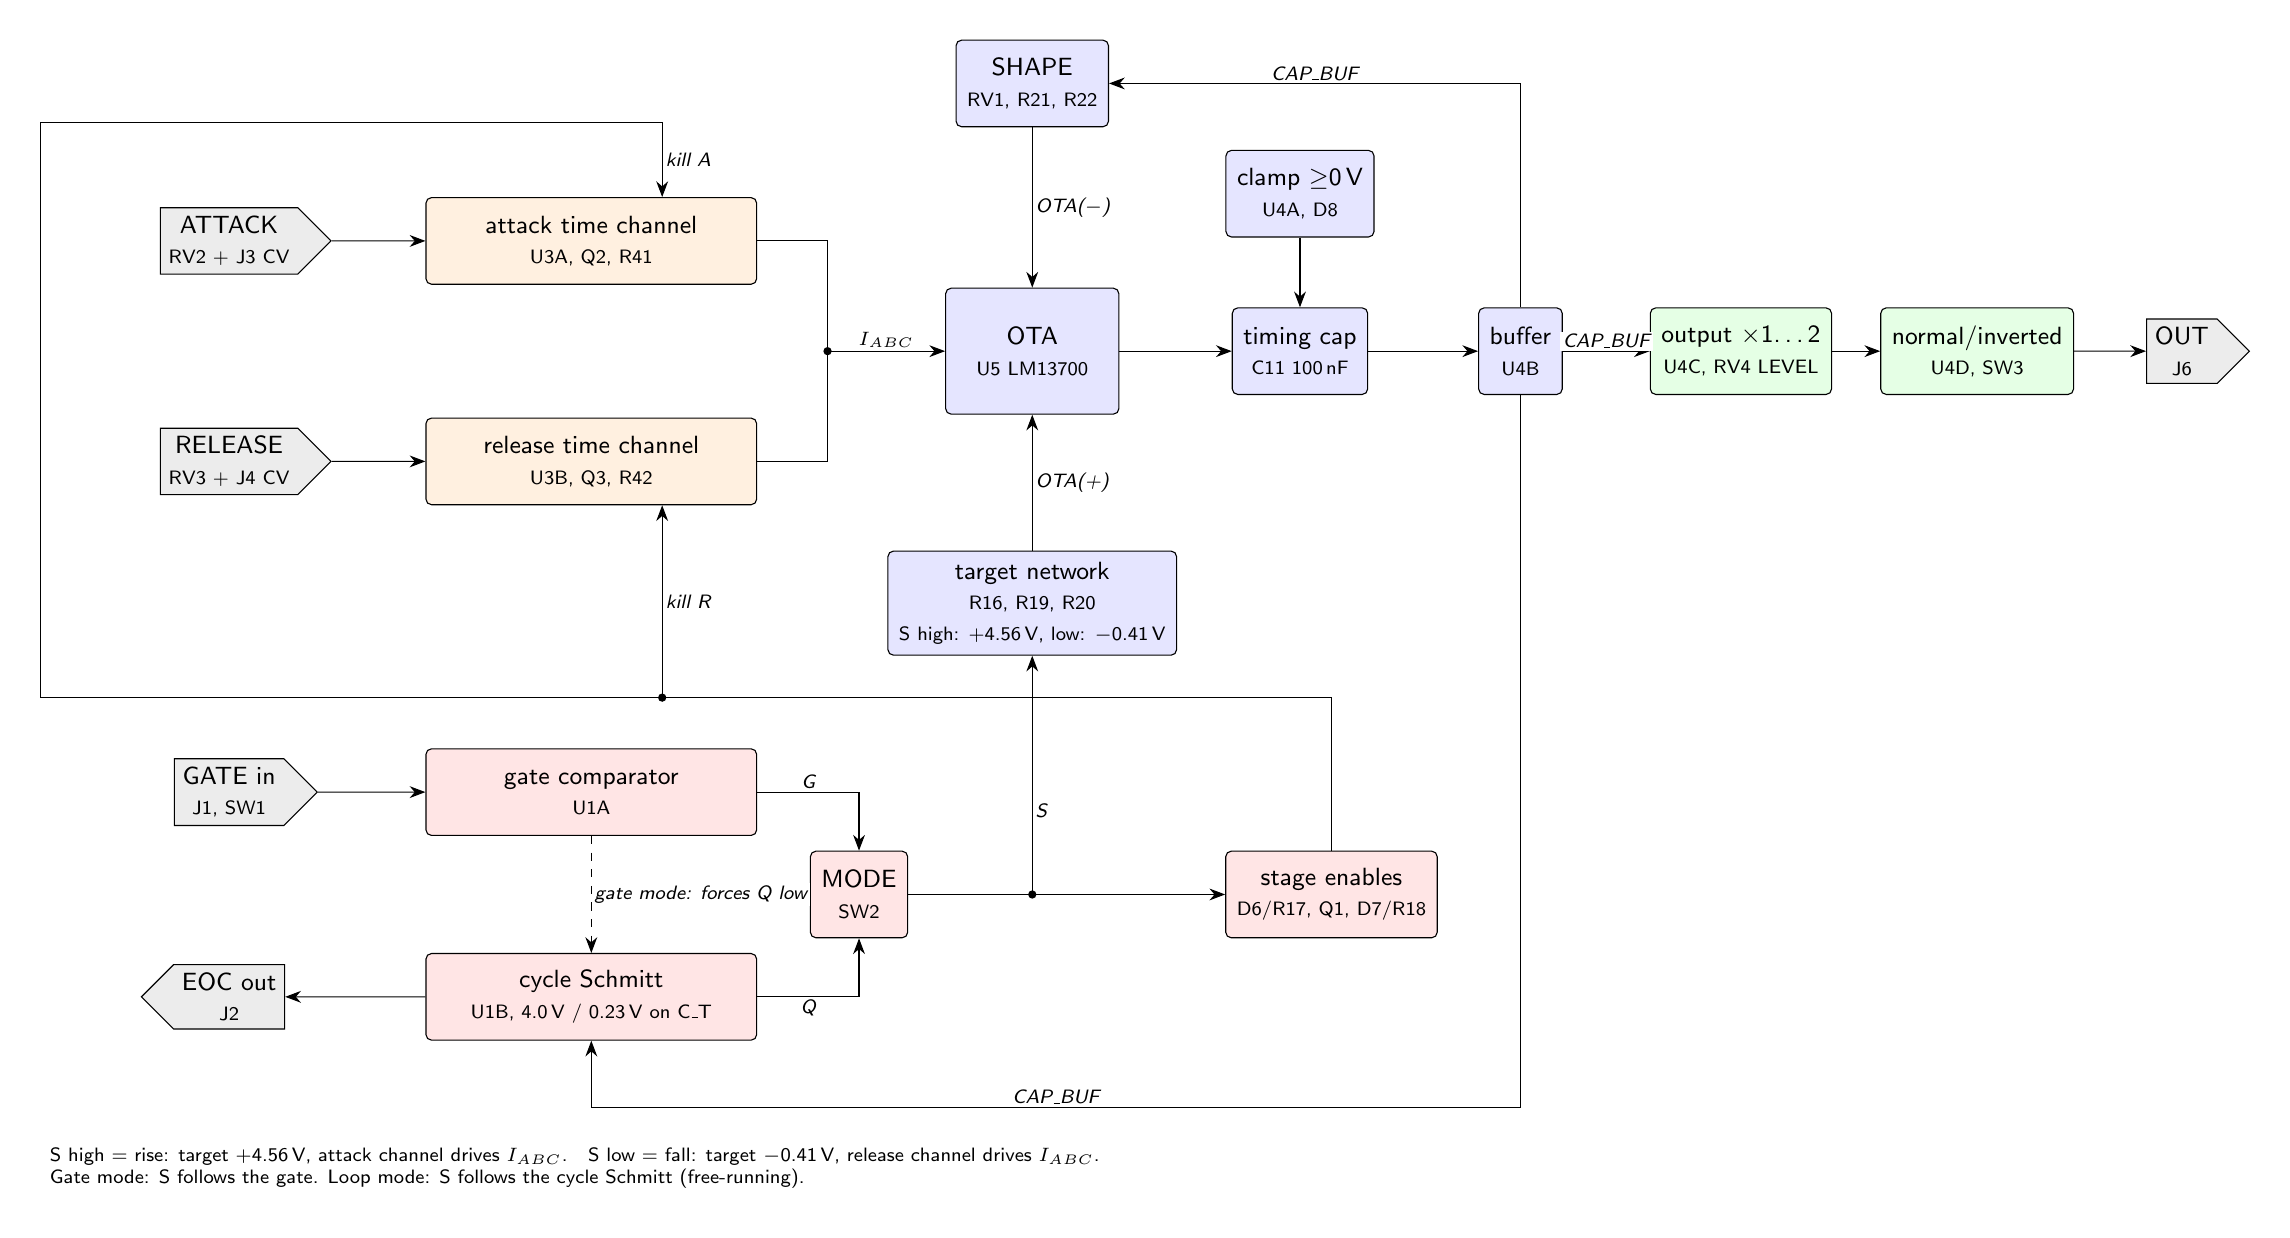
\begin{tikzpicture}[font=\sffamily\small, >={Stealth[length=2mm]},
    show background rectangle, background rectangle/.style={fill=white},
    blk/.style={draw, rounded corners=2pt, align=center, minimum height=11mm, inner sep=4pt, fill=#1},
    blk/.default=white,
    io/.style={draw, signal, signal to=east, fill=gray!15, minimum height=7mm, inner sep=3pt, align=center},
    ioL/.style={io, signal to=west},
    sig/.style={font=\sffamily\scriptsize\itshape, fill=white, inner sep=1pt}]

  % ---------------- timing ----------------
  \node[blk=orange!12, minimum width=42mm] (ta) at (0, 1.4) {attack time channel\\\scriptsize U3A, Q2, R41};
  \node[blk=orange!12, minimum width=42mm] (tr) at (0,-1.4) {release time channel\\\scriptsize U3B, Q3, R42};
  \node[io] (pa) at (-4.6, 1.4) {ATTACK\\\scriptsize RV2 + J3 CV};
  \node[io] (pr) at (-4.6,-1.4) {RELEASE\\\scriptsize RV3 + J4 CV};
  \draw[->] (pa) -- (ta);
  \draw[->] (pr) -- (tr);

  % ---------------- core ----------------
  \node[blk=blue!10, minimum width=22mm, minimum height=16mm] (ota) at (5.6,0) {OTA\\\scriptsize U5 LM13700};
  \draw (ta.east) -- (3.0,1.4) -- (3.0,-1.4) -- (tr.east);
  \draw[->] (3.0,0) -- node[sig, above]{$I_{ABC}$} (ota.west);
  \fill (3.0,0) circle (1.5pt);
  \node[blk=blue!10] (ct) at (9.0,0) {timing cap\\\scriptsize C11 100\,nF};
  \node[blk=blue!10] (cl) at (9.0,2.0) {clamp $\geq$0\,V\\\scriptsize U4A, D8};
  \node[blk=blue!10] (buf) at (11.8,0) {buffer\\\scriptsize U4B};
  \node[blk=green!10] (outs) at (14.6,0) {output $\times$1\ldots2\\\scriptsize U4C, RV4 LEVEL};
  \node[blk=green!10] (inv) at (17.6,0) {normal/inverted\\\scriptsize U4D, SW3};
  \node[io] (out) at (20.2,0) {OUT\\\scriptsize J6};
  \draw[->] (ota) -- (ct);
  \draw[->] (cl) -- (ct);
  \draw[->] (ct) -- (buf);
  \draw[->] (buf) -- node[sig, above]{CAP\_BUF} (outs);
  \draw[->] (outs) -- (inv);
  \draw[->] (inv) -- (out);

  % shape (feedback, above) and target (below)
  \node[blk=blue!10] (shape) at (5.6,3.4) {SHAPE\\\scriptsize RV1, R21, R22};
  \draw[->] (buf.north) |- node[sig, pos=.75, above]{CAP\_BUF} (shape.east);
  \draw[->] (shape) -- node[sig, right]{OTA($-$)} (ota);
  \node[blk=blue!10] (tgt) at (5.6,-3.2) {target network\\\scriptsize R16, R19, R20\\\scriptsize S high: +4.56\,V, low: $-$0.41\,V};
  \draw[->] (tgt) -- node[sig, right]{OTA(+)} (ota);

  % ---------------- logic ----------------
  \node[io] (gin) at (-4.6,-5.6) {GATE in\\\scriptsize J1, SW1};
  \node[blk=red!10, minimum width=42mm] (gc) at (0,-5.6) {gate comparator\\\scriptsize U1A};
  \node[blk=red!10, minimum width=42mm] (sch) at (0,-8.2) {cycle Schmitt\\\scriptsize U1B, 4.0\,V / 0.23\,V on C\_T};
  \node[ioL] (eoc) at (-4.6,-8.2) {EOC out\\\scriptsize J2};
  \node[blk=red!10] (mode) at (3.4,-6.9) {MODE\\\scriptsize SW2};
  \node[blk=red!10] (en) at (9.4,-6.9) {stage enables\\\scriptsize D6/R17, Q1, D7/R18};
  \draw[->] (gin) -- (gc);
  \draw[->] (gc.east) -| node[sig, pos=.25, above]{G} (mode.north);
  \draw[->] (sch.east) -| node[sig, pos=.25, below]{Q} (mode.south);
  \draw[->] (sch) -- (eoc);
  \draw[->, dashed] (gc) -- node[sig, right]{gate mode: forces Q low} (sch);
  \draw (mode) -- (5.6,-6.9);
  \fill (5.6,-6.9) circle (1.5pt);
  \draw[->] (5.6,-6.9) -- node[sig, pos=.35, right]{S} (tgt);
  \draw[->] (5.6,-6.9) -- (en);
  % kill lines to the time channels
  \draw[->] (en.north) |- (0.9,-4.4) -- node[sig, pos=.5, right]{kill R} (0.9,-1.4 |- tr.south);
  \fill (0.9,-4.4) circle (1.5pt);
  \draw[->] (0.9,-4.4) -| (-7.0,2.9) -| node[sig, pos=.75, right]{kill A} (0.9,1.4 |- ta.north);
  % CAP_BUF to the Schmitt
  \draw[->] (buf.south) |- node[sig, pos=.75, above]{CAP\_BUF} (0,-9.6) -- (sch.south);

  \node[font=\sffamily\scriptsize, align=left, anchor=north west] at (-7.0,-10.0)
    {S high = rise: target +4.56\,V, attack channel drives $I_{ABC}$.\quad
     S low = fall: target $-$0.41\,V, release channel drives $I_{ABC}$.\\
     Gate mode: S follows the gate. Loop mode: S follows the cycle Schmitt (free-running).};
\end{tikzpicture}
\end{document}
